
\begin{frame}{Специальная часть}
    \center{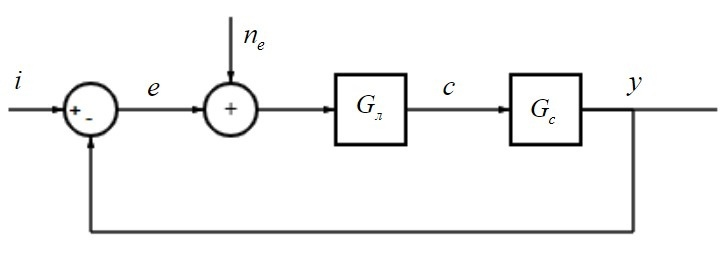
\includegraphics[width=11cm, height = 6cm]{../Оглавление/Part3/figures/СамолётЛётчик.png}}
\end{frame}
\begin{frame}{Специальная часть}{Линеаризованная модель объкта управления}
    \begin{equation} \begin{aligned} \dot{x} = Ax+Bu \\ 
    y = Cx + Du \end{aligned} \end{equation}
$$\dot{x} = \begin{bmatrix}
        \dot{V}_x\\ 
        \dot{V}_y\\ 
        \dot{\omega_z}\\ 
        \dot{\theta}
    \end{bmatrix},
u = \delta_\text{э}$$
   $ A = \begin{bmatrix}
        -0.0110 & 0.0433 & 1.7295 & -7.1876\\ 
        -0.0691 & -0.6975 & -7.0678 & -54.8976\\ 
        0.00011 & 0.00116 & -0.35407 & 0.0911\\ 
        0 & 0 & 1 & 0
    \end{bmatrix} ,$  
        $B = \begin{bmatrix}
        -0.4412\\ 
        -12.388\\ 
        -0.58446 \\ 
        0
    \end{bmatrix}$  
\end{frame}

\begin{frame}{Специальная часть}{Робастность системы}
    \begin{block}{Схема}
        \center{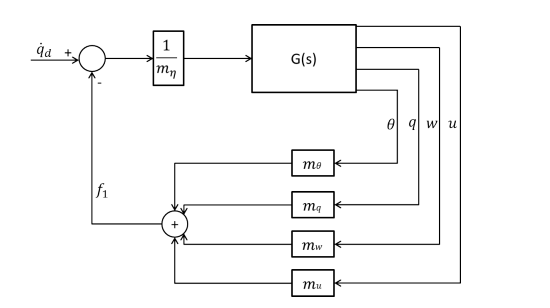
\includegraphics[width=11cm, height = 6cm]{../Оглавление/Part3/figures/Неполная схема СПС.png}}
    \end{block}
\end{frame}
 
\begin{frame}{Специальная часть}{Робастность системы}
    \begin{block}{Коэффициенты}
        \begin{center}
    $m_\theta = 0.0911$ \\
    $m_{V_x} = 0.00011$ \\ 
    $m_{V_y} = 0.0016$ \\ 
    $m_{\omega_z} = -0.35407$ \\ 
    $m_{\delta_\text{э}} = -0.58446$ \\ 
        \end{center}
    \end{block}
    $$\delta_\text{э}= -\frac{1}{m_{\delta_\text{э}}} (m_{\omega_z} \omega_z + m_{V_y} V_y + m_{V_x} V_x - \dot{\omega}_z)$$ 
\end{frame}

\begin{frame}{Специальная часть}{Робастность системы}
    \begin{block}{Результаты экспериментов}
        \center{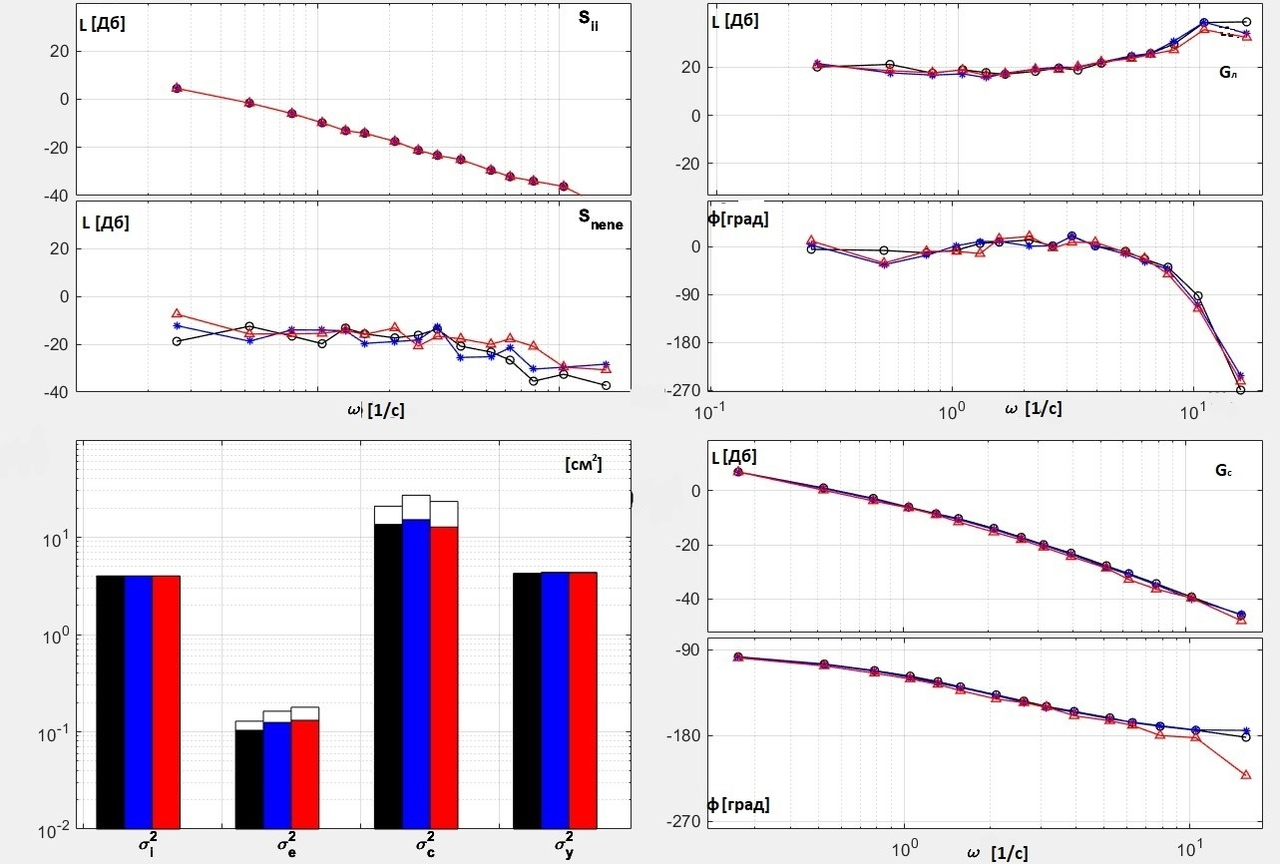
\includegraphics[width=11cm, height = 6cm]{../Оглавление/Part3/figures/Модель без PI.jpg}}
    \end{block}
\end{frame}

\begin{frame}{Специальная часть}{Робастность системы}

\begin{table}[H]
    \begin{tabular}{|c|c|c|c|}
        \hline 
        № э.& $\sigma^2_e,$ см$^2$ & $\sigma^2_c$ см$^2$ & $n_e$ см$^2$ \\ \hline 
        1& 0.103 & 13.54 & 0.0254\\ \hline
        2& 0.125 & 15.14  & 0.037 \\ \hline
        3& 0.131 & 12.74 & 0.047\\ \hline

    \end{tabular}
\end{table}
\end{frame}
 
\begin{frame}{Специальная часть}{Робастность системы}
\begin{table}[H]
    \begin{tabular}{|c|c|c|c|c|}
        \hline 
        № э.&Нули & Полюса & $\xi$ & $\omega_c$, 1/c \\ \hline 
        1& -2 & - & 1.0 &0.5 \\ \hline
        & -1.9392 & -0.7537  &  & 1.59 $\cdot 10^{-4}$\\ 
        2& -0.7473 & -0.0161  &1.0 & 1.64 $\cdot 10^{-2}$\\ 
        & -0.0164 &  0 & &7.47 $\cdot 10^{-1}$\\ 
        & 0 &   &  &1.94 \\ \hline 
        & -1.8207 & 0.8255 & &0\\ 
        3& -0.8033 & -0.0177 & 1.0&1.85 $\cdot 10^{-2}$\\ 
        & -0.0185 & 0 & &8.03 $\cdot 10^{-1}$ \\ 
        & 0 &  &  &1.82 \\ \hline
    \end{tabular}
\end{table}

\end{frame}

\begin{frame}{Специальная часть}{Параметры PI-контроллера}
    \begin{block}{Задача PI-контроллера}
        PI-котроллер в теории должен уменьшать  
    \end{block}
    \begin{block}{PI-короллер}
        $$y(t) = K_p + \frac{1}{p}K_i,$$
        где $K_p = 2$, $K_i = 5$.
        Коэффициенты PI-котроллера были выбраны с условием того, что система должна оставаться устойчева.     
    \end{block}
\end{frame}

\begin{frame}{Специальная часть}{Улучшение робасности с применением PI-контроллера}
    \begin{block}{Схема}
        \center{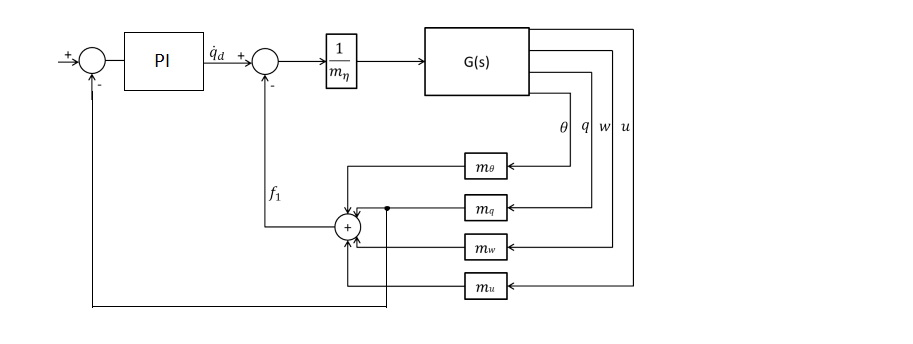
\includegraphics[width=10cm, height = 6cm]{../Оглавление/Part3/figures/Полная схема СПС.png}}
    \end{block}
\end{frame}

\begin{frame}{Специальная часть}{Улучшение робасности с применением PI-контроллера}
    \begin{block}{Результаты экспериментов}
        \center{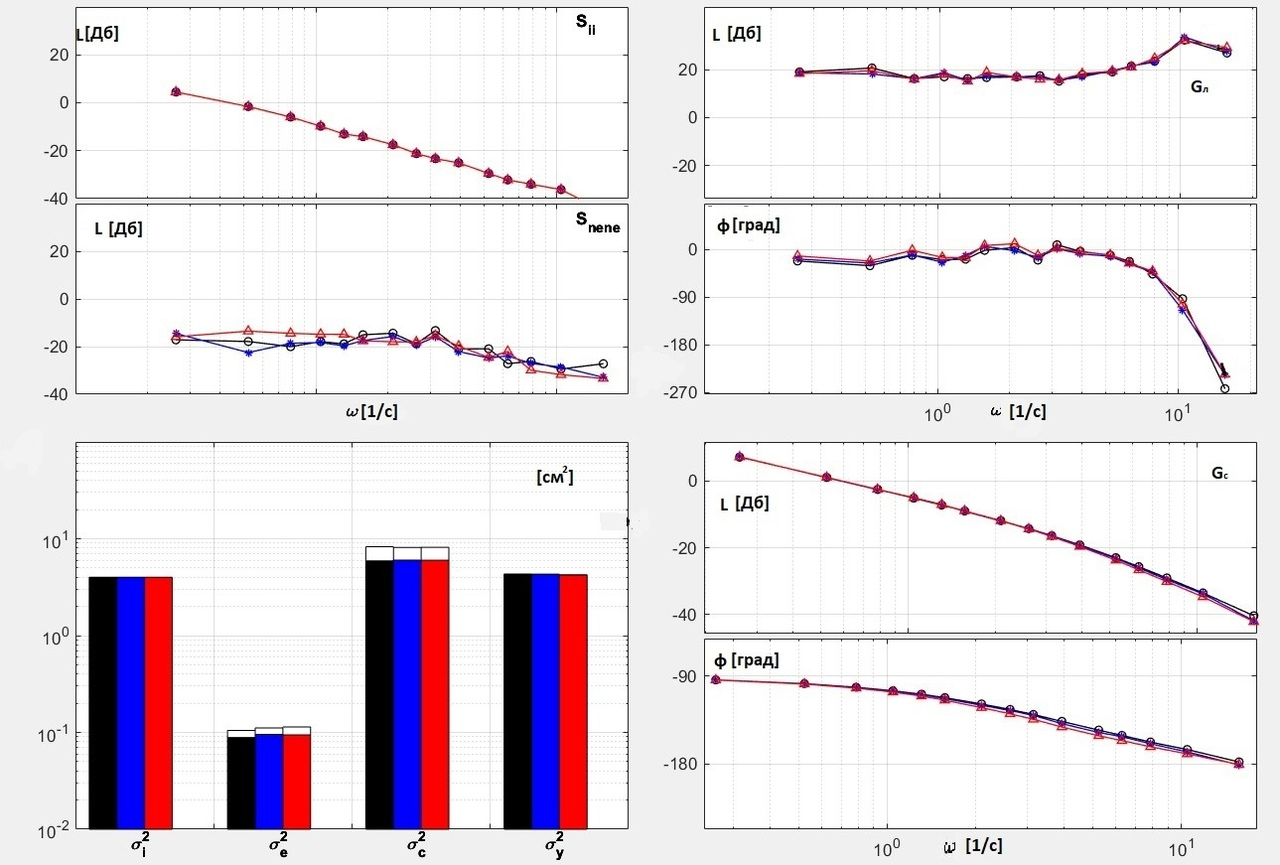
\includegraphics[width=11cm, height = 6cm]{../Оглавление/Part3/figures/Модель с PI.jpg}}
    \end{block}
\end{frame}


\begin{frame}{Специальная часть}{Робастность системы}

\begin{table}[H]
    \begin{tabular}{|c|c|c|c|}
        \hline 
        № э.& $\sigma^2_e,$ см$^2$ & $\sigma^2_c$ см$^2$ & $n_e$ см$^2$ \\ \hline 
        1& 0.0886 & 5.913 & 0.01611\\ \hline
        2& 0.0952 & 6.01  & 0.01591 \\ \hline
        3& 0.0943 & 6.004 & 0.01712\\ \hline

    \end{tabular}
\end{table}
\end{frame}
 
\begin{frame}{Специальная часть}{Робастность системы}
\begin{table}[H]
    \begin{tabular}{|c|c|c|c|c|}
        \hline 
        № э.&Полюса & Нули & $\xi$ & $\omega_c$, 1/c \\ \hline 
        1& -3.0000 + 1.0000$i$ & -2.5 & 0.95 & 3.16\\ 
        & -3.0000 - 1.0000$i$ &   &  &  \\ \hline
        2& -2.8660 + 1.1287$i$ & -0.0161  & 1.0 &  0\\ 
        & -2.8660 - 1.1287$i$ &  -0.7537 &1.0 & 1.61$\cdot 10^{-2}$\\ 
        & -0.7547 + 0.0000$i$ &  -2.5000 & 1.0 & 7.51 $\cdot 10^{-2}$\\ 
        & 0 & 0.0000 & 0.93& 3.08 \\ 
        & -0.0161 + 0.0000$i$ &  & 0.93 &  \\ \hline 
        3& -2.5975 + 1.3096$i$ & -0.0177 & 1 & 0\\ 
        & -2.5975 - 1.3096$i$ & -0.8255 & 1& 1.77 $\cdot 10^{-2}$ \\ 
        & -0.8292 + 0.0000$i$ & -2.5000 & 1 & 8.29 $\cdot 10^{-1}$\\ 
        & 0 & 0 & 0.893 & 2.91 \\ 
        & -0.0177 + 0.0000$i$ &  &  &  \\ \hline 
    \end{tabular}
\end{table}
\end{frame}

\begin{frame}{Специальная часть}{Переходные процессы}
    \begin{minipage}[c]{0.45\textwidth}
        \center{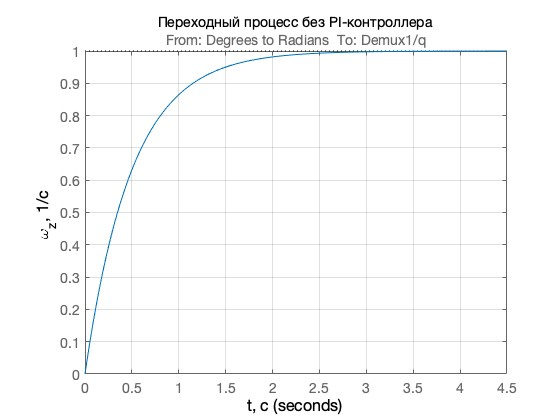
\includegraphics[width=6cm, height = 6cm]{img/withoutPI.jpg}}
    \end{minipage}
    \begin{minipage}[c]{0.45\textwidth}
        \center{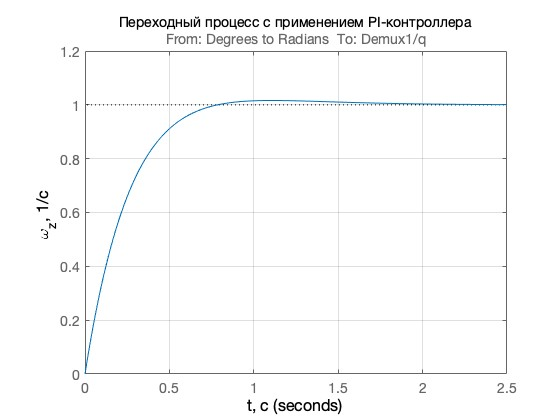
\includegraphics[width=6cm, height = 6cm]{img/withPI.jpg}}
    \end{minipage}
\end{frame}
